\chapter{信号调理与滤波器}
\label{chap:hw-conditioning}

\noindent 本章对应《课后作业—信号调理与滤波》的全部6题。电桥计算先约定接法，频谱计算先约定横轴与谱线高度，滤波计算逐频率处理；各题的知识扩展均由原题所用原理展开。


\needspace{11\baselineskip}
\section{第1题：单臂与双臂电桥的输出和灵敏度}
\label{hw:5-1}
\keypoint{复习重点：微应变先换算；先求电阻变化，再分别代入精确桥路公式。}

\begin{hwquestion}
电阻应变片的初始阻值 $R=120\,\Omega$，灵敏系数 $S_g=2$；其余固定电阻初始也为 $120\,\Omega$，供桥电压 $U_0=3\,\mathrm V$，负载电阻视为无穷大。当应变分别为 $\varepsilon=2\,\mu\varepsilon$、$2000\,\mu\varepsilon$ 时，求单臂、双臂电桥的输出电压，并比较灵敏度。
\end{hwquestion}

\subsection*{答案与解析}
\textbf{桥路接法与符号约定。}电源接桥的上、下端，上端电势 $U_0$、下端为0。左支路上臂为 $R_2$、下臂为 $R_1$，其中点记为 $d$；右支路上臂为 $R_3$、下臂为 $R_4$，其中点记为 $b$。取输出 $U_y=V_d-V_b$，则
\[
U_y=U_0\left(\frac{R_1}{R_1+R_2}-\frac{R_4}{R_3+R_4}\right).
\]
单臂取 $R_1$ 增大，其余不变；双臂取相邻的 $R_1$ 增大、$R_2$ 等量减小，其余两臂固定，因此对正应变均得到正输出。原题未给出双臂的受力布置，这里采用常见的等量拉压半桥。

\textbf{第一步：把应变换成电阻相对变化。}
\[
\delta=\frac{\Delta R}{R}=S_g\varepsilon.
\]
当 $\varepsilon=2\times10^{-6}$ 时，$\delta=4\times10^{-6}$、$\Delta R=0.00048\,\Omega$；当 $\varepsilon=2000\times10^{-6}=0.002$ 时，$\delta=0.004$、$\Delta R=0.48\,\Omega$。

\textbf{第二步：单臂采用精确分压式。}
\begin{align*}
U_{y,1}&=U_0\left(\frac{R+\Delta R}{2R+\Delta R}-\frac12\right)\\
&=\boxed{\frac{U_0\Delta R}{4R+2\Delta R}
=\frac{U_0\delta}{4+2\delta}}.
\end{align*}
代入两种应变：
\begin{align*}
U_{y,1}(2\,\mu\varepsilon)
&=\frac{3\times4\times10^{-6}}{4+8\times10^{-6}}\,\mathrm V
\approx\boxed{2.999994\,\mu\mathrm V},\\
U_{y,1}(2000\,\mu\varepsilon)
&=\frac{3\times0.004}{4+0.008}\,\mathrm V
\approx\boxed{2.994012\,\mathrm{mV}}.
\end{align*}
小信号近似 $U_{y,1}\approx U_0\delta/4$ 分别给出 $3\,\mu\mathrm V$ 与 $3\,\mathrm{mV}$。

\textbf{第三步：双臂让相邻电阻等量反向变化。}
\begin{align*}
U_{y,2}&=U_0\left(\frac{R+\Delta R}{(R+\Delta R)+(R-\Delta R)}-\frac12\right)\\
&=\boxed{\frac{U_0\Delta R}{2R}=\frac{U_0\delta}{2}}.
\end{align*}
分母精确保持 $2R$，所以无需舍去高阶项：
\[
\boxed{U_{y,2}(2\,\mu\varepsilon)=6\,\mu\mathrm V},\qquad
\boxed{U_{y,2}(2000\,\mu\varepsilon)=6\,\mathrm{mV}}.
\]

\begin{table}[H]
\centering\small
\begin{tabular}{@{}c c c c@{}}
\toprule
应变 & 单臂精确输出 & 单臂线性近似 & 双臂精确输出 \\
\midrule
$2\,\mu\varepsilon$ & $2.999994\,\mu\mathrm V$ & $3\,\mu\mathrm V$ & $6\,\mu\mathrm V$ \\
$2000\,\mu\varepsilon$ & $2.994012\,\mathrm{mV}$ & $3\,\mathrm{mV}$ & $6\,\mathrm{mV}$ \\
\bottomrule
\end{tabular}
\end{table}

\textbf{第四步：明确比较哪一种灵敏度。}零点小信号灵敏度为
\[
K_{\varepsilon,1}(0)=\frac{U_0S_g}{4}
=1.5\,\mathrm{\mu V}/\mu\varepsilon,
\qquad
K_{\varepsilon,2}=\frac{U_0S_g}{2}
=3\,\mathrm{\mu V}/\mu\varepsilon.
\]
双臂为单臂的2倍，并在理想等量反向条件下保持精确线性。若比较非零输入处的局部斜率，单臂应取导数：
\[
K_{\varepsilon,1}(\varepsilon)
=\frac{U_0S_g}{4(1+S_g\varepsilon/2)^2},\qquad
\frac{K_{\varepsilon,2}}{K_{\varepsilon,1}(\varepsilon)}
=2(1+S_g\varepsilon/2)^2.
\]
而 $U_y/\varepsilon$ 是从零点到测量点的\textbf{割线灵敏度}，对非线性单臂桥并不等于局部导数。直接比较两种输出的比值为 $U_{y,2}/U_{y,1}=2+\delta$，分别为 $2.000004$ 与 $2.004$；它与“零点灵敏度之比为2”并不矛盾。

\textbf{第五步：量化单臂桥路非线性。}以线性化输出为基准定义偏差
\[
e_{\mathrm{nl}}=\frac{U_{y,1}-U_{y,1}^{\mathrm{lin}}}{U_{y,1}^{\mathrm{lin}}}
=-\frac{\delta}{2+\delta}.
\]
两点分别约为 $-0.000200\%$ 与 $-0.199601\%$。若以精确输出为分母，线性近似的相对高估为 $\delta/2$，分别是 $0.000200\%$ 与 $0.200000\%$；误差分母不同，数值也略有不同。

\nt{此处双臂结果假定两片分别受等量拉、压应变。如果两片相邻且同向变化，理想输出会抵消。单臂桥输出的正负还取决于接线；换接输出端后，上述所有电压反号，灵敏度大小不变。}

\subsection*{本题知识点与公式}\label{kn:5-1}
\noindent\textbf{已学前置：}应变 $\varepsilon=\Delta l/l$、应变片灵敏系数 $S_g$ 及 $\Delta R/R=S_g\varepsilon$ 见\hyperref[kn:4-1]{第4章第1题知识讲解}。\textbf{本题新增：}完整学习电桥怎样把电阻变化转为电压，包括桥臂位置、接法与输出灵敏度。

\paragraph{1. 电桥来自两个分压器，平衡就是两个中点等电势}
在答案约定的接法中，电源跨接上、下端，两条支路分别为 $R_2$ 与 $R_1$ 串联、$R_3$ 与 $R_4$ 串联。输出端开路时，每条支路电流只由本支路总电阻决定。由欧姆定律，
\[
I_L=\frac{U_0}{R_1+R_2},\quad V_d=I_LR_1,\qquad
I_R=\frac{U_0}{R_3+R_4},\quad V_b=I_RR_4.
\]
中点电势相减得到任意四臂的\textbf{精确开路输出}：
\[
\boxed{\frac{U_y}{U_0}
=\frac{R_1R_3-R_2R_4}{(R_1+R_2)(R_3+R_4)}}.
\]
所以电桥平衡条件是 $R_1R_3=R_2R_4$，不要求四个阻值全部相等。等臂桥 $R_i=R$ 是最常见的平衡特例。电阻以 $\Omega$ 计，电压以V计，$U_y/U_0$ 为无量纲比值，常以 $\mathrm{mV/V}$ 报告。上述分压式假设电源电压已知、输出无电流；有负载时不能把两条支路仍看作互不影响的分压器。

\paragraph{2. 小信号线性化怎样确定四臂的正负号}
令 $R_i=R(1+\delta_i)$、$|\delta_i|\ll1$。利用
$(1+z)^{-1}=1-z+O(z^2)$，左中点的归一化电势为
\[
\frac{1+\delta_1}{2+\delta_1+\delta_2}
=\frac12+\frac{\delta_1-\delta_2}{4}+O(\delta^2).
\]
右中点同理为 $1/2+(\delta_4-\delta_3)/4+O(\delta^2)$，故
\[
\boxed{\frac{U_y}{U_0}\approx
\frac14(\delta_1-\delta_2+\delta_3-\delta_4)}.
\]
$\delta_i=\Delta R_i/R$ 无量纲；$O(\delta^2)$ 表示二次及更高阶小量。这里的“相邻臂异号、对臂同号”指\textbf{同一个电阻增量对所选输出的贡献符号}。交换输出端会使全部符号反转，但不改变输出大小。本题单臂增大 $R_1$ 得正输出；相邻的 $R_2$ 若减小，其负号与负增量相乘，贡献便与 $R_1$ 相加。

\paragraph{3. 单臂、双臂和全桥的倍数有接法条件}
\begin{center}\small
\begin{tabularx}{\linewidth}{@{}p{1.4cm}Xp{3cm}@{}}
\toprule
接法 & 电阻相对变化与受力条件 & $U_y/U_0$\\
\midrule
单臂 & $\delta_1=\delta$，其余为0 & $\delta/(4+2\delta)\approx\delta/4$\\
拉压双臂 & $\delta_1=\delta,\ \delta_2=-\delta$，其余为0 & $\delta/2$\\
交替全桥 & $\delta_1=\delta_3=\delta,\ \delta_2=\delta_4=-\delta$ & $\delta$\\
\bottomrule
\end{tabularx}
\end{center}
三者的零点应变灵敏度为 $U_0S_g/4,\ U_0S_g/2,\ U_0S_g$，所以有常用的 $1:2:4$ 倍数。双臂和全桥的表中结果在各支路总电阻不变、应变--电阻关系线性的条件下是精确的。若两个相邻臂同向等量变化，二者分压比保持 $1/2$，输出抵消；同向变化的两片若接在对臂，其小信号贡献则可相加，不能只凭“有两片”就指定倍数。

\textbf{泊松半桥不是等量拉压半桥。}若同一试件表面一片沿轴向、一片沿横向，处于单轴应力且横向可自由收缩，横向应变为 $-\nu_p\varepsilon$。$\nu_p$ 为无量纲泊松比，两片同 $S_g$ 并接相邻臂时，
\[
\frac{U_y}{U_0}
=\frac{(1+\nu_p)S_g\varepsilon}
       {4+2(1-\nu_p)S_g\varepsilon}
\approx\frac{(1+\nu_p)S_g}{4}\varepsilon.
\]
它一般不等于 $S_g\varepsilon/2$；受约束、多轴应力或横向灵敏度明显时，还须修正模型。本题答案采用的是弯曲等场景中的等量拉压布置。

\paragraph{4. 温度补偿补偿的是共同变化}
若相邻两片的温度增量均为 $\delta_T$，而有效应变只作用于工作片，则 $\delta_1=\delta_\varepsilon+\delta_T$、$\delta_2=\delta_T$，小信号输出中的 $\delta_T$ 相消。补偿片须与工作片温度接近、温度特性匹配且不承受所测应变；若两片还同时承受同向有效应变，有效信号也会被抵消。引线电阻不等、温度梯度与片间不一致会留下残差，不能把“半桥”本身视为无条件温度补偿。

\paragraph{5. 有限输入阻抗要用戴维南等效}
把桥的输出等效为开路电压 $U_{\mathrm{oc}}$ 与串联电阻 $R_{\mathrm{th}}$。求 $R_{\mathrm{th}}$ 时将理想电压源短路，两个中点各自看到一组并联电阻，因此
\[
R_{\mathrm{th}}=(R_1\parallel R_2)+(R_3\parallel R_4),
\qquad R_a\parallel R_b=\frac{R_aR_b}{R_a+R_b}.
\]
负载 $R_L$ 跨接两中点时，
\[
\boxed{U_L=U_{\mathrm{oc}}\frac{R_L}{R_L+R_{\mathrm{th}}}}.
\]
等臂初始桥有 $R_{\mathrm{th}}=R$；$R_L\gg R_{\mathrm{th}}$ 时才接近开路值。加载衰减随桥臂变化还可能引入附加非线性。本题 $R_L\to\infty$ 正是允许直接使用分压结果的条件。交流桥需把电阻换成复阻抗，并同时满足幅值、相位平衡，见\hyperref[kn:4-2]{第4章第2题知识讲解}。

\paragraph{6. 灵敏度、非线性与供桥电压应分开评价}
局部灵敏度 $K_\varepsilon=\diff U_y/\diff\varepsilon$ 描述某工作点附近的增量；割线灵敏度 $[U_y(\varepsilon)-U_y(0)]/\varepsilon$ 描述从零到该点的平均变化。它们的单位为V/单位应变，也可用 $\mu\mathrm V/\mu\varepsilon$；电阻式应变片的 $S_g$ 则无量纲。单臂精确式可展开为
\[
\frac{U_y}{U_0}
=\frac{\delta}{4}\left(1-\frac{\delta}{2}
+\frac{\delta^2}{4}-\cdots\right).
\]
首个被舍去的电压项为 $-U_0\delta^2/8$，解释了本题大应变点的输出略小于线性值。相对误差必须说明分母，答案给出的两种百分比不能混用。

提高 $U_0$ 能按比例提高电压灵敏度，却不改变理想桥的相对非线性。在平衡等臂桥中，每片两端电压为 $U_0/2$，耗散功率为 $P_i=U_0^2/(4R)$，单位W；自热随供桥电压的平方增加。实际桥压还要满足应变片散热、功耗及放大器输入范围，不能只追求输出电压大。

\needspace{11\baselineskip}
\section{第2题：全桥交流激励的输出及三组频谱}
\label{hw:5-2}
\keypoint{复习重点：全桥的相邻臂必须等量反向；本题所有时间系数均为角频率。}

\begin{hwquestion}
用四片电阻应变片组成全桥，测量
\[
\varepsilon(t)=A\cos10t+B\cos100t.
\]
激励电压为 $u_0(t)=E\sin10000t$，求电桥输出，并画出测量信号、激励信号、输出信号的频谱。
\end{hwquestion}

\subsection*{答案与解析}
\textbf{先说明全桥条件。}原题未给应变片灵敏系数，保留为 $S_g$，并假设四片相同。令 $\delta(t)=S_g\varepsilon(t)$，且
\[
R_1=R_3=R[1+\delta(t)],\qquad
R_2=R_4=R[1-\delta(t)].
\]
即一组对臂受拉、另一组对臂受等量压缩。代入桥路分压式：
\begin{align*}
u_y(t)&=u_0(t)\left[\frac{1+\delta(t)}2-\frac{1-\delta(t)}2\right]\\
&=\boxed{S_gE[A\cos10t+B\cos100t]\sin10000t}.
\end{align*}
该式在电阻--应变关系线性、四臂等量交替变化及高输入阻抗条件下为精确桥路结果。若四片同向等量变化，分压比均不变，不会得到此输出。

\textbf{展开乘积，直接读出四条正频率边带。}
\begin{align*}
u_y(t)=\frac{S_gEA}{2}\bigl[\sin10010t+\sin9990t\bigr]\\
\hspace{1.2cm}+\frac{S_gEB}{2}\bigl[\sin10100t+\sin9900t\bigr].
\end{align*}
注意这里用的是 $\sin\omega_ct\cos\Omega t$，且 $\omega_c>\Omega$，上下两边带均可写成正幅值正弦项。应变信号无直流分量，所以理想输出中\textbf{没有单独位于 $10000\,\mathrm{rad/s}$ 的载波线}。

\textbf{建立明确的双边谱线约定。}本题用复指数线谱
\[
v(t)=\sum_{\nu}C_{\nu}e^{\iu\nu t}
\]
表示周期信号，横轴为角频率 $\nu$。其中
\[
M\cos\nu t\ \longleftrightarrow\ C_{+\nu}=C_{-\nu}=\frac M2,
\]
\[
M\sin\nu t\ \longleftrightarrow\ C_{+\nu}=\frac{M}{2\iu}=-\iu\frac M2,
\quad C_{-\nu}=\iu\frac M2.
\]
若采用角频率傅里叶变换 $V_\omega(\omega)=\int v(t)e^{-\iu\omega t}\diff t$，则其冲激权重是 $2\pi C_\nu$，即
$V_\omega(\omega)=2\pi\sum_\nu C_\nu\delta(\omega-\nu)$。\textbf{谱线系数与傅里叶冲激权重不能混用。}

\begin{table}[H]
\centering\small
\begin{tabularx}{\linewidth}{@{}p{1.25cm} p{3.7cm} X@{}}
\toprule
信号 & 正角频率 $\nu$（$\mathrm{rad/s}$） & 对应的正频率复系数 $C_{+\nu}$ \\
\midrule
应变 & $10$；$100$ & $A/2$；$B/2$ \\
激励 & $10000$ & $-\iu E/2$ \\
输出 & $9990,\ 10010$ & 两条均为 $-\iu S_gEA/4$ \\
输出 & $9900,\ 10100$ & 两条均为 $-\iu S_gEB/4$ \\
\bottomrule
\end{tabularx}
\end{table}
所有信号为实信号，故负频率系数由 $C_{-\nu}=C_{+\nu}^{*}$ 给出。若 $A,B,E,S_g>0$，应变各线相位为零；激励及输出的正频率线相位均为 $-90^\circ$，负频率线为 $+90^\circ$。若 $A$ 或 $B$ 为负，相应谱线再反相 $180^\circ$。

\begin{center}
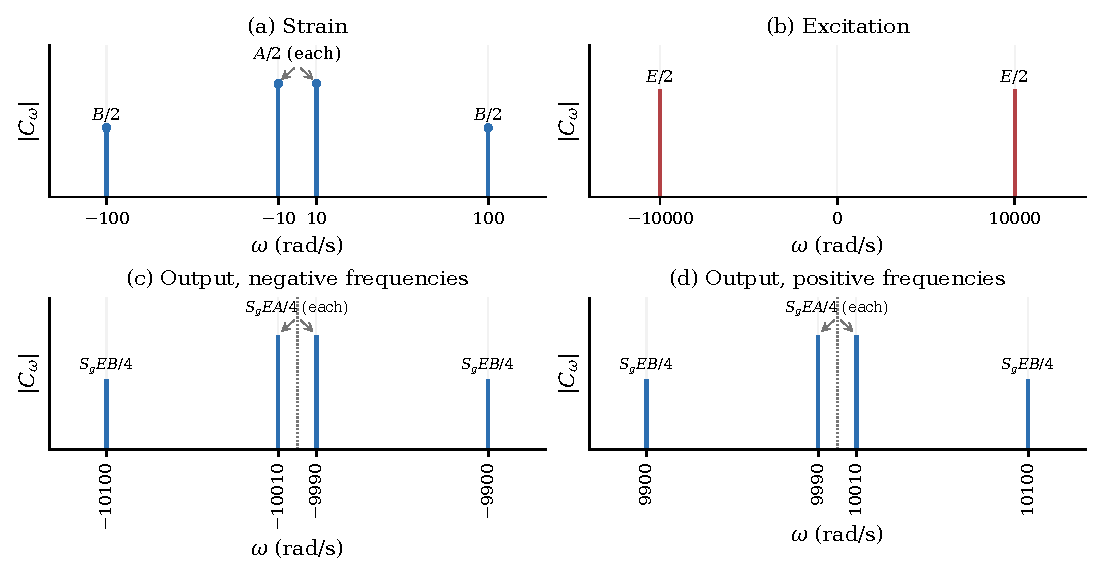
\includegraphics[width=.98\linewidth]{ch5-bridge-spectra.pdf}
\end{center}
图画的是双边复系数的模 $|C_\nu|$，纵向高度按符号示意，精确值见标注；输出正负频率簇分开展示，实际频率位置保持不变。虚线标出载频，虚线位置没有理想谱线。

\textbf{与Hz频谱的换算。}各频率都除以 $2\pi$。激励频率是
\[
f_c=\frac{10000}{2\pi}\approx1591.55\,\mathrm{Hz},
\]
并非 $10\,\mathrm{kHz}$。应变两频率约为 $1.592$、$15.915\,\mathrm{Hz}$，边带相对载频的偏移也分别是这两个数值。

\nt{只给单边峰值谱时，两组输出边带的高度分别为 $|S_gEA|/2$ 与 $|S_gEB|/2$。本题图采用双边复系数模，因此相应高度再减半。无论采用哪一种，都必须说明约定，并保留正弦激励所决定的相位信息。}

\subsection*{本题知识点与公式}\label{kn:5-2}
\noindent\textbf{已学前置：}桥臂接法和全桥系数见\hyperref[kn:5-1]{本章第1题知识讲解}；乘余弦的频移性质见\hyperref[kn:2-6]{第2章第6题知识讲解}；冲激缩放见\hyperref[kn:2-3]{第2章第3题知识讲解}。本题新增交流应变桥的乘法模型、实际桥谱的三种表示对照，以及带参考相位误差的同步解调。

\paragraph{1. 桥路的分压比为何成为调幅系数}
电桥的电源是交流量，并不意味着每个桥臂都必须是电抗。本题桥臂为电阻，若其瞬时电阻由缓变应变确定、导线电容等寄生效应可忽略，原来的电阻分压公式在每个时刻仍成立。设 $k_b$ 为无量纲桥路系数，则
\[
u_y(t)=k_bS_g\varepsilon(t)u_0(t).
\]
等量拉压双臂 $k_b=1/2$，交替全桥 $k_b=1$；单臂 $k_b=1/4$ 仅为小信号近似。$S_g,\varepsilon$ 无量纲，$u_0,u_y$ 单位为V，故系数量纲闭合。若桥臂含电抗、激励频率已使寄生参数显著，就要用交流阻抗桥模型，而不能把此瞬时乘法式当作精确结论。

取 $u_0=E\sin\omega_ct$，令 $K_b=k_bS_gE$，有 $u_y=K_b\varepsilon\sin\omega_ct$。$K_b$ 的单位为V/单位应变。应变控制载波幅值，其变号使输出相对激励反相 $180^\circ$；这正是测量拉、压方向的信息。本题全桥 $K_b=S_gE$，故不能额外再除以4。

记 $\mathcal E(f)=\int_{-\infty}^{\infty}\varepsilon(t)e^{-\iu2\pi ft}\diff t$ 为应变的Hz傅里叶变换（周期信号按广义线谱理解）。

\paragraph{2. 双边带抑制载波的“抑制”指无独立载波线}
设应变频谱限于 $|f|\leq f_m$，载频 $f_c=\omega_c/(2\pi)>f_m$。正弦载波的Hz频谱为
\[
U_y(f)=\frac{K_b}{2\iu}
\left[\mathcal E(f-f_c)-\mathcal E(f+f_c)\right].
\]
正、负载频附近各有一份搬移后的基带谱，每份带有幅值和相位系数；正频率簇占 $[f_c-f_m,f_c+f_m]$。本题应变无直流，因而在 $\pm f_c$ 处无单独谱线，称为双边带抑制载波调幅（DSB-SC）。若应变有直流偏置，该偏置乘载波会产生载频谱线，不能仍断言载波线必为零。

本题 $f_m=100/(2\pi)\,\mathrm{Hz}$，而不是100 Hz；输出所需通带是所有边带的位置范围。实信号的负频率系数为正频率系数的共轭，负频率不表示出现另一套独立的物理振荡。

\paragraph{3. 对本题桥谱统一三种表示}
\hyperref[kn:2-6]{第2章第6题}已经定义傅里叶级数系数。把本题任一周期信号写成
$v(t)=\sum_kC_ke^{\iu\nu_kt}$，其中 $\nu_k$ 为角频率、$f_k=\nu_k/(2\pi)$。同一信号的表示对照为
\begin{center}\small
\begin{tabularx}{\linewidth}{@{}p{2.7cm}X>{\raggedright\arraybackslash}p{2.8cm}@{}}
\toprule
表示法 & 在正频率线的位置与系数 & 本题正弦项 $M\sin\nu_kt$\\
\midrule
复指数线谱 & $\nu_k$ 或 $f_k$ 处画 $C_k$ & $C_k=-\iu M/2$\\
Hz傅里叶变换 & $V_f(f)=\sum_kC_k\delta(f-f_k)$ & 冲激权重 $-\iu M/2$\\
角频率傅里叶变换 & $V_\omega(\omega)=2\pi\sum_kC_k\delta(\omega-\nu_k)$ & 冲激权重 $-\iu\pi M$\\
\bottomrule
\end{tabularx}
\end{center}
两种连续变换的关系是 $V_\omega(\omega)=V_f(\omega/2\pi)$。对冲激代入时必须用
\[
\delta\!\left(\frac{\omega}{2\pi}-f_k\right)
=2\pi\,\delta(\omega-2\pi f_k).
\]
因此“横轴从Hz改成rad/s”若指连续傅里叶谱，冲激权重也出现 $2\pi$；若指把同一组傅里叶级数系数移到角频率坐标，$C_k$ 本身不变。这个因子来自变量缩放，正好对应角频率反变换中的 $1/(2\pi)$。

若 $v$ 是电压，$C_k$ 与单边峰值的单位为V，连续傅里叶变换整体的量纲为 $\mathrm{V\,s}$；冲激箭头标的是权重，不是有限高度的“谱密度”。本题每个输出正弦峰值为 $S_gEA/2$ 或 $S_gEB/2$，所以图中的 $|C_k|$ 分别为其一半，正频率相位为 $-90^\circ$。这同时核对了答案表、频谱图与时域展开，不能只对位置而漏对系数。

\paragraph{4. 同步乘法为什么能恢复应变符号}
用同频参考 $r(t)=B_r\sin(\omega_ct+\theta)$，这里将参考作为无量纲控制量，$B_r$ 为无量纲参考幅值，$\theta$ 为参考相对信号载波的相差；真实电压乘法器还须计入其转换系数。由积化和差，
\[
u_yr=\frac{K_bB_r}{2}\varepsilon(t)
\left[\cos\theta-\cos(2\omega_ct+\theta)\right].
\]
低通除去 $2\omega_c$ 附近的频谱后，
\[
\boxed{v_{\mathrm{LP}}(t)
=\frac{K_bB_r}{2}\cos\theta\,\varepsilon(t)}.
\]
参考同相时恢复有符号的基带；$\theta=90^\circ$ 时有效输出为零；$\theta=180^\circ$ 时输出反号。小相差以弧度计时 $\cos\theta\approx1-\theta^2/2$，会形成比例误差。若参考另有频率偏差 $\Delta\omega$，低频项会乘 $\cos(\Delta\omega t+\theta)$，产生缓慢起伏，不能由固定增益校准消除。

高频副本的最低正频率为 $2f_c-f_m$，因此理想分离要求低通保留 $|f|\leq f_m$，并抑制 $2f_c$ 附近的副本；$f_c>f_m$ 提供了不重叠的条件。实际滤波器还要留过渡带，并满足基带内的幅相精度。普通包络只反映 $|K_b\varepsilon|$，拉压符号丢失；同步参考使这个符号可以保留下来。本题之后第4题将把桥、交流放大、解调和低通合并成整条测量链。

\needspace{11\baselineskip}
\section{第3题：多频调幅波的分量与频谱}
\label{hw:5-3}
\keypoint{复习重点：括号中的直流产生载波，余弦分量各产生一对边带。}

\begin{hwquestion}
已知
\[
x_a(t)=(100+30\cos\Omega t+20\cos3\Omega t)\cos\omega_ct,
\]
其中 $f_c=10\,\mathrm{kHz}$、$f_\Omega=500\,\mathrm{Hz}$。求各分量的频率与幅值，并画出调制信号与调幅波的频谱。
\end{hwquestion}

\subsection*{答案与解析}
把零均值的信息信号记为 $m(t)=30\cos\Omega t+20\cos3\Omega t$，把实际控制载波幅值的量记为 $q(t)=100+m(t)$。二者的区别只有 $q$ 含直流100；称“调制信号”时须明确指哪一个。

\textbf{第一步：展开为五个余弦。}
\begin{align*}
x_a(t)={}&100\cos\omega_ct\\
&+15\cos(\omega_c-\Omega)t+15\cos(\omega_c+\Omega)t\\
&+10\cos(\omega_c-3\Omega)t+10\cos(\omega_c+3\Omega)t.
\end{align*}
因此，$30$与$20$是信息信号的峰值，各自平均分到上下两个边带。

\begin{table}[H]
\centering
\begin{tabular}{@{}c c c@{}}
\toprule
分量 & 频率（$\mathrm{kHz}$） & 时域余弦峰值 \\
\midrule
三倍调制频率的下边带 & $10-1.5=8.5$ & $10$ \\
基频的下边带 & $10-0.5=9.5$ & $15$ \\
载波 & $10$ & $100$ \\
基频的上边带 & $10+0.5=10.5$ & $15$ \\
三倍调制频率的上边带 & $10+1.5=11.5$ & $10$ \\
\bottomrule
\end{tabular}
\end{table}

\textbf{第二步：给出带直流的调制量频谱。}沿用Hz傅里叶变换约定：
\[
Q(f)=100\delta(f)+15[\delta(f-500)+\delta(f+500)]
+10[\delta(f-1500)+\delta(f+1500)].
\]
若画的是 $m(t)$，删去 $100\delta(f)$，其余完全相同。调幅后
\begin{align*}
X_a(f)={}&50[\delta(f-10000)+\delta(f+10000)]\\
&+7.5\!\!\sum_{\nu\in\{9500,10500\}}[\delta(f-\nu)+\delta(f+\nu)]\\
&+5\!\!\sum_{\nu\in\{8500,11500\}}[\delta(f-\nu)+\delta(f+\nu)].
\end{align*}
每条正、负频率线的冲激权重是对应余弦峰值的一半；各系数为正，故相位均为零。

\begin{center}
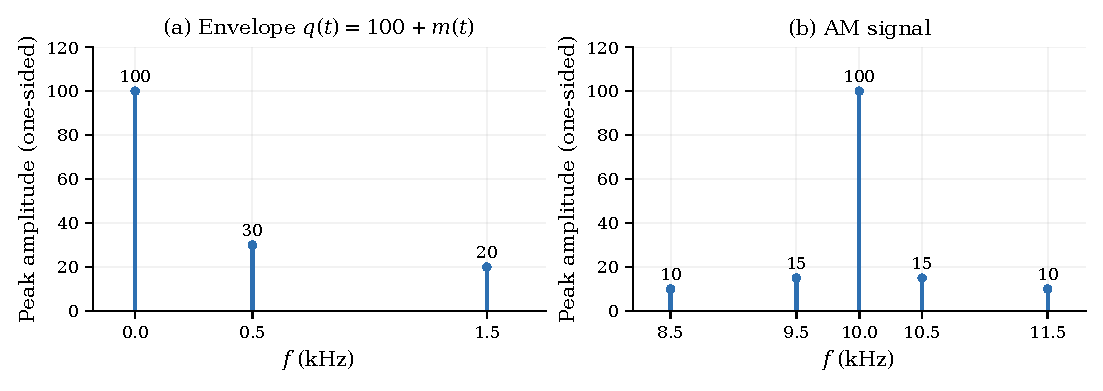
\includegraphics[width=.98\linewidth]{ch5-am-spectra.pdf}
\end{center}
为方便直接读取五个余弦的幅值，本图使用\textbf{单边峰值谱}：正频率余弦项画其峰值，直流画其常数值。若改画双边谱，在正负两侧各画一半峰值；直流仍为100，不做翻倍或减半。

\textbf{第三步：检验包络是否翻折。}由三角不等式，
\[
q(t)\geq100-30-20=50>0.
\]
因而该调幅波无包络翻折，可在适当时间常数与器件工作条件下采用包络检波，检出 $q(t)$ 后再去掉直流100。正频率占用范围为 $8.5\sim11.5\,\mathrm{kHz}$，带宽为 $3\,\mathrm{kHz}=2\times1500\,\mathrm{Hz}$。

\nt{直流100不产生“零频率的射频输出”，而是乘载波后形成 $10\,\mathrm{kHz}$ 谱线。$3\Omega$ 对应 $1500\,\mathrm{Hz}$，不能把它当作 $3\,\mathrm{Hz}$，也不能把两个边带幅值仍写成30、20。}

\subsection*{本题知识点与公式}\label{kn:5-3}
\noindent\textbf{已学前置：}频谱搬移见\hyperref[kn:2-6]{第2章第6题}；本章第\ref{hw:5-2}节已讲DSB-SC和三种线谱约定。本题新增带独立载波的常规调幅、多音调制度、包络检波条件及同阻抗下的功率分配。

\paragraph{1. 常规AM把直流偏置也乘到了载波上}
令零均值信息为 $m(t)$、偏置为 $D>0$，常规AM写成
\[
x_a(t)=[D+m(t)]\cos\omega_ct,\qquad
m(t)=\sum_iM_i\cos(\Omega_it+\theta_i).
\]
$D$ 与 $M_i$ 的量纲相同；若 $x_a$ 为电压，它们以V计。展开后，$D\cos\omega_ct$ 是独立载波，每个调制分量产生
\[
\frac{M_i}{2}\cos[(\omega_c+\Omega_i)t+\theta_i]
+\frac{M_i}{2}\cos[(\omega_c-\Omega_i)t-\theta_i].
\]
此处假设 $\omega_c>\Omega_i>0$。下边带的相位为 $-\theta_i$，上边带为 $+\theta_i$，不能在有初相位时只复制幅值而忽略相位。本题初相位全为0，因此五个余弦分量均可按正峰值直接读谱。

Hz变换中，正频率载波冲激权重是 $D/2$，第 $i$ 组正频率上、下边带的复权重分别为 $(M_i/4)e^{\iu\theta_i}$、$(M_i/4)e^{-\iu\theta_i}$，其模均为 $|M_i|/4$；单边峰值谱则画 $D$ 与 $|M_i|/2$。信息谱本身在 $\pm f_i$ 的复权重为 $(M_i/2)e^{\pm\iu\theta_i}$。搬移的一次减半与双边分解的一次减半各有来源，不能因此丢掉谱线相位。

\paragraph{2. 多音调制度应怎样定义与检查}
单音时定义无量纲调制度 $\mu=|M|/D$。多音可逐项记 $\mu_i=|M_i|/D$，但是否过调取决于总和 $m(t)$ 的实际最小值：
\[
\boxed{D+m(t)\geq0\quad\text{对全部 }t\text{ 成立}}.
\]
一个便于手算的充分条件是
\[
D\geq\sum_i|M_i|\qquad\Longleftrightarrow\qquad
\sum_i\mu_i\leq1.
\]
它利用了三角不等式；相位或频率关系使极小值不能同时出现时，这个条件可以偏保守，不能把“超过此充分界限”一概当作已经证明过调。对多音只检验每个 $\mu_i<1$ 也不充分，因为各项可能同时向下叠加。

本题 $\mu_1=0.3,\ \mu_3=0.2$，且总和为0.5，故 $q(t)=100+m(t)$ 始终为正。理想外包络为 $|q(t)|$；当 $q$ 不变号时，它保留全部调制波形。若 $q$ 变负，外包络会把负部翻上来，丢失有符号的 $q$，造成包络检波失真；已有相干参考时仍可用同步方法恢复，这是解调方式的条件，而非乘法公式失效。

\paragraph{3. 带宽由最高调制频率决定}
当信息频谱占 $|f|\leq f_m$、载频 $f_c>f_m$ 时，正载频附近的边带范围为 $f_c-f_m$ 到 $f_c+f_m$，所需传输带宽为
\[
\boxed{B_{\mathrm{AM}}=2f_m}.
\]
$B_{\mathrm{AM}}$ 与 $f_c$ 均以Hz计，$\omega_c$ 与 $\Omega_i$ 则以rad/s计。本题最高调制频率是 $3f_\Omega=1500\,\mathrm{Hz}$，所以传输带宽为3000 Hz。独立载波线位于此区间中间；它的存在不再额外增加占用带宽。

\paragraph{4. 载波与边带的平均功率从正交性得到}
以下专指 $x_a$ 为电压、作用在同一纯电阻负载 $R_L$ 上、各谱线频率互不重合，且按足够长时间或共同周期求平均。峰值为 $V_p$ 的余弦均方根为 $|V_p|/\sqrt2$，平均功率为 $V_p^2/(2R_L)$。不同频率交叉项平均为零，故载波与全部边带功率分别为
\[
P_c=\frac{D^2}{2R_L},\qquad
P_{\mathrm{SB}}=\sum_i2\frac{(M_i/2)^2}{2R_L}
=\frac{\sum_iM_i^2}{4R_L}.
\]
功率以W计，$R_L$ 以 $\Omega$ 计。总功率与信息边带所占比例为
\[
P_{\mathrm{tot}}=P_c\left(1+\frac12\sum_i\mu_i^2\right),
\qquad
\eta=\frac{P_{\mathrm{SB}}}{P_{\mathrm{tot}}}
=\frac{\sum_i\mu_i^2}{2+\sum_i\mu_i^2}.
\]
这也可由\hyperref[kn:2-6]{第2章第6题的Parseval关系}得到。载波提供包络偏置，却本身不随信息变化；因而常规AM的功率并非全部位于信息边带。单音不过调时 $\mu\leq1$，此模型的最高边带功率比例为 $1/3$。多音不能把 $\sum\mu_i^2$ 直接当作包络极值条件，功率求和与峰值叠加是不同问题。若各频率看到不同阻抗，上式需要逐频率计算真实功率，不能只比较电压平方。

\paragraph{5. 包络检波还需要时间尺度与器件条件}
理想二极管--RC检波器在载波峰附近充电，峰间通过负载放电：时间常数太小会留下明显载波纹波，太大则跟不上下降包络。常用量级条件是
\[
\frac1{\omega_c}\ll\tau_d\ll\frac1{\omega_m},
\qquad \omega_m=2\pi f_m.
\]
$\tau_d$ 单位为s。这只是载波与包络快慢分离的指导式；实际还须检查允许纹波、二极管压降、充电时间及斜切失真。下降包络的局部跟随还要求放电速率不小于包络下降速率，即近似检查
$q/\tau_d\gtrsim|\diff q/\diff t|$。因此即使本题已经证明不过调，也不能跳过检波器动态条件。检出 $q(t)$ 后，去除已知直流 $D$ 并标定增益，才得到零均值信息 $m(t)$。

\needspace{11\baselineskip}
\section{第4题：激励频率与动态应变仪工作频带}
\label{hw:5-4}
\keypoint{复习重点：载频是搬移位置，工作频率是可准确恢复的被测量频带。}

\begin{hwquestion}
某动态应变仪的电桥激励频率为 $10\,\mathrm{kHz}$，工作频率为 $0\sim1500\,\mathrm{Hz}$。用调幅与解调原理解释二者的关系。
\end{hwquestion}

\subsection*{答案与解析}
设应变频谱限于 $|f|\leq1500\,\mathrm{Hz}$，理想桥路输出 $u_y(t)=K\varepsilon(t)\cos(2\pi10000t)$，则
\[
U_y(f)=\frac K2[\mathcal E(f-10000)+\mathcal E(f+10000)].
\]
其中 $\mathcal E(f)$ 为应变频谱，$K$ 含桥路系数、片灵敏系数与激励幅值。因此输出在正载频附近占
\[
\boxed{10000-1500\leq f\leq10000+1500}
\quad\Longrightarrow\quad\boxed{8.5\sim11.5\,\mathrm{kHz}}.
\]
交流放大与带通环节应覆盖整段边带。同步乘以同相 $10\,\mathrm{kHz}$ 参考后，信号一部分回到 $0\sim1500\,\mathrm{Hz}$ 基带，另一部分移到 $20\,\mathrm{kHz}$ 附近。低通保留基带，再作比例标定，便得到应变输出。

所以\textbf{10 kHz是激励载频，1500 Hz是被测应变变化频率的上限}。工作频带受桥路、交流放大、解调和输出低通的整体幅相特性约束，并不是由激励频率直接等同得到。

\textbf{下限为何可为零？}恒定应变会改变载波幅值或相对相位，仍能由同步或相敏检波恢复为有正负的直流输出。只要测量链允许直流基带，就能测静态应变；信息不要求必须以低频电压直接通过全部交流放大级。

\textbf{带宽检查：}两边带共需3000 Hz带宽；输出低通还需在0--1500 Hz内满足精度，不能把1500 Hz直接当作无误差的 $-3\,\mathrm{dB}$ 截止点。

\subsection*{本题知识点与公式}\label{kn:5-4}
\noindent\textbf{已学前置：}频谱搬移与同步解调见\hyperref[kn:5-2]{本章第2题}，包络与有符号信息的区别见\hyperref[kn:5-3]{本章第3题}。本题新增整条动态应变测量链的通带要求，以及载频附近的响应怎样共同决定基带测量精度。

\paragraph{1. 沿测量链追踪同一段信息}
交流供桥的基本链路是
\[
\text{应变}\ \longrightarrow\ \text{交流桥调幅}\
\longrightarrow\ \text{带通放大}\
\longrightarrow\ \text{同步解调}\
\longrightarrow\ \text{输出低通}.
\]
信号在各环节的频谱位置不同，但被测应变的变化频率没有因此变成载频。设应变占 $|f|\leq f_m$，桥输出采用 $K\varepsilon(t)\cos2\pi f_ct$，则正载频附近占 $[f_c-f_m,f_c+f_m]$。本题 $f_c=10\,\mathrm{kHz}$、$f_m=1.5\,\mathrm{kHz}$，因而各环节应检查：
\begin{center}\small
\begin{tabularx}{\linewidth}{@{}p{2.5cm}X@{}}
\toprule
环节 & 需要通过或抑制的频带\\
\midrule
交流桥与交流放大 & 正频率有效边带为 $8.5\sim11.5\,\mathrm{kHz}$，负频率为其镜像；幅相均须满足恢复要求。\\
同步乘法 & 同频参考把有效信息搬回 $|f|\leq1.5\,\mathrm{kHz}$，同时产生 $2f_c$ 附近副本。\\
输出低通 & 保留 $0\sim1.5\,\mathrm{kHz}$，并抑制 $18.5\sim21.5\,\mathrm{kHz}$ 的正频率副本及其负频率镜像。\\
\bottomrule
\end{tabularx}
\end{center}
真实电路还会产生谐波和噪声，表中范围描述理想乘法所需的最低频谱检查。本题不能据此确定实际电路的阶数或允许误差，因为这些指标没有给出。

\paragraph{2. 为什么不能只检查载频处的增益}
把桥后、解调前的线性响应记为 $G(f)$，输出低通记为 $L(f)$，二者均为复数频响。无量纲参考取 $2\cos(2\pi f_ct+\theta)$；系数2专门补偿一次乘余弦的 $1/2$。设带外副本最终被低通除去，则由两次频移直接得到基带等效频响
\[
\boxed{
H_{\mathrm{eq}}(f)=\frac K2 L(f)
\left[e^{-\iu\theta}G(f+f_c)+e^{\iu\theta}G(f-f_c)\right]
},\qquad |f|\leq f_m.
\]
推导要点是：第一次调制产生的两份 $\mathcal E$，经过 $G$ 后分别乘上各自所在频率处的响应；第二次调制把它们都搬到基带，因此\textbf{复数贡献相加}，不能只相加幅值。这一公式假定激励稳定、桥路乘法模型成立、带外副本不与基带重叠，并且参考与载波同频。若参考未乘系数2，整式还要再除以2。

$K$ 的单位为V/单位应变；若其余环节输出、输入都是电压，$G,L$ 为无量纲增益，$H_{\mathrm{eq}}$ 仍是V/单位应变。实系数电路满足 $G(-f)=G^*(f)$，但正载频附近上下边带的增益、相位仍可能不对称；只在 $f_c$ 测一个增益不能知道整个 $H_{\mathrm{eq}}$ 是否平坦。

若边带范围内 $G$ 等效于共同增益与延迟，并通过参考相位校准消除载波传播相移，基带可近似得到一个共同增益和共同延迟。若上下边带的幅相畸变不同，一个参考相位旋钮一般不能补偿全部基带频率。

\paragraph{3. 工作频带、通带指标与截止频率的区别}
“工作频率 $0\sim1500\,\mathrm{Hz}$”应理解为在规定精度下可测的应变变化范围。完整指标还应给允许幅值误差、相位误差或延迟误差。设用直流灵敏度 $H_{\mathrm{eq}}(0)>0$ 标定，并允许共同延迟 $t_d$，可用
\[
\left|\frac{|H_{\mathrm{eq}}(f)|}{H_{\mathrm{eq}}(0)}-1\right|
\leq\epsilon_A,\qquad
\left|\arg H_{\mathrm{eq}}(f)+2\pi ft_d\right|
\leq\epsilon_\phi
\]
检查工作频带内的保真性；相位须先连续展开，$\epsilon_A$ 无量纲，$\epsilon_\phi$ 用rad，$t_d$ 用s。单频幅值测量可能只规定第一项，多频波形测量则不能忽略第二项。

半功率截止点的幅值已经降到参考值的 $1/\sqrt2$，即约29.3\%衰减，通常不等于精密测量的带宽边界。对一阶输出低通，若要求在 $f_m$ 处衰减不超过 $\epsilon_A$，由\hyperref[kn:3-2]{第3章第2题}可直接写出
\[
\tau\leq
\frac{\sqrt{(1-\epsilon_A)^{-2}-1}}{2\pi f_m},
\qquad
f_{\mathrm{cut}}\geq
\frac{f_m}{\sqrt{(1-\epsilon_A)^{-2}-1}}.
\]
所以实际设计需让允许误差内的通带覆盖1500 Hz，并另给过渡带；不能把 $f_{\mathrm{cut}}=1500\,\mathrm{Hz}$ 当作默认答案。第5题将统一讲截止与滤波器的其他频带指标。

\paragraph{4. 交流放大为何仍能测零频率应变}
恒定应变 $\varepsilon_0$ 使桥输出为 $K\varepsilon_0\cos2\pi f_ct$，它是载频处的交流信号，能够通过交流放大级。同步解调后得到与 $\varepsilon_0$ 成正比的直流，因此\textbf{被测量的零频率不需要以直流电压穿过解调前的全部电路}。

要保留直流与符号，必须保证解调参考相位稳定、最终基带链有非零直流增益、后级不再用去直流高通把静态信息删去，并且正负应变的标定一致。按\hyperref[kn:5-2]{第2题}，参考相差会给基带乘 $\cos\theta$：相差 $90^\circ$ 会使有效信号消失，反相会使拉压符号颠倒。实际零点漂移与桥路初始失衡还需单独调零；调零并不等于可以丢掉被测量真实的直流变化。

\nt{本题激励 $10\,\mathrm{kHz}$ 与第2题的 $10000\,\mathrm{rad/s}$ 是不同单位、不同数值；不能把二者直接当作同一个载频。}

\needspace{11\baselineskip}
\section{第5题：截止频率与倍频程判断}
\label{hw:5-5}
\keypoint{复习重点：从 $f_{c2}/f_{c1}=2^n$ 推导，避免把三个不同的根号混淆。}

\begin{hwquestion}
设带通滤波器下、上截止频率为 $f_{c1},f_{c2}$，中心频率为 $f_0$。判断：
\begin{enumerate}
\item 一倍频程滤波器有 $f_{c2}=\sqrt2\,f_{c1}$。
\item $f_0=\sqrt{f_{c1}f_{c2}}$。
\item 截止频率位于幅值相对通带参考值下降约 $3\,\mathrm{dB}$ 的位置。
\item 下限频率相同时，一倍频程中心频率为 $1/3$ 倍频程中心频率的 $\sqrt[3]2$ 倍。
\end{enumerate}
\end{hwquestion}

\subsection*{答案与解析}
本题采用对数对称带通频带和常用半功率截止点约定。

\textbf{（1）错误。}一倍频程的定义是上下限频率之比为2：
\[
\boxed{f_{c2}=2f_{c1}},\qquad
f_0=\sqrt{f_{c1}\cdot2f_{c1}}=\sqrt2\,f_{c1}.
\]
命题把中心与下限之比，误写成上限与下限之比。若上、下限比为 $\sqrt2=2^{1/2}$，相应宽度只有半倍频程。

\textbf{（2）正确。}对数轴上的中点满足
\[
\log f_0=\frac{\log f_{c1}+\log f_{c2}}2,
\]
所以 $f_0=\sqrt{f_{c1}f_{c2}}$，不是算术平均 $(f_{c1}+f_{c2})/2$。该结论使用了本题的中心频率定义。

\textbf{（3）按本题常用约定正确。}半功率点的幅值比是 $1/\sqrt2$，
\[
20\log_{10}\frac{1}{\sqrt2}=-3.0103\,\mathrm{dB}\approx-3\,\mathrm{dB}.
\]
须相对于规定通带参考幅值；它不是绝对电压的分贝读数。采用其他截止指标的滤波器，需使用对应定义。

\textbf{（4）正确。}设共同下限为 $f_L$。一倍频程上限为 $2f_L$，中心为 $2^{1/2}f_L$；$1/3$ 倍频程上限为 $2^{1/3}f_L$，中心为 $2^{1/6}f_L$。故
\[
\boxed{\frac{f_{0,\,1\mathrm{oct}}}{f_{0,\,1/3\mathrm{oct}}}
=2^{1/2-1/6}=2^{1/3}=\sqrt[3]2}.
\]


\subsection*{本题知识点与公式}\label{kn:5-5}
\noindent\textbf{已学前置：}测量精度内的工作频带与截止点的区别见\hyperref[kn:5-4]{本章第4题}；一阶幅相曲线见\hyperref[kn:3-1]{第3章第1题}。本题新增滤波器的完整频带语言、分贝和滚降，以及对数对称带通的中心、品质因子与倍频程关系。

\paragraph{1. 四种滤波器按“允许通过什么”区分}
对线性时不变滤波器，$Y(f)=H(f)X(f)$，$H$ 一般同时改变幅值与相位。对实系数滤波器，实冲激响应保证 $H(-f)=H^*(f)$，负频率响应由此确定，通常只列正频率：
\begin{center}\small
\begin{tabularx}{\linewidth}{@{}p{1.3cm}p{3.2cm}X@{}}
\toprule
类型 & 主要通过范围 & 本章中的联系\\
\midrule
低通 & 从直流到某上边界 & 同步解调后保留应变基带。\\
高通 & 高于某下边界 & 可抑制直流漂移；但不能用于必须保留静态应变的最终基带。\\
带通 & 下、上边界之间 & 在载频附近保留两边带并抑制较远干扰。\\
带阻 & 通过某段阻带以外的频率 & 抑制窄频段干扰；阻带很窄时常称陷波。\\
\bottomrule
\end{tabularx}
\end{center}
滤波能按频率选择成分；有用信号与噪声若处于相同频率，普通线性选频不能只除去噪声而保留该频率的全部信号。需要保留波形时，也不能只画幅频响应而完全不检查相位。

\paragraph{2. 通带、阻带、过渡带与截止点是不同指标}
通带是在规定最大衰减或纹波内通过的范围；阻带是在规定最小衰减下需抑制的范围；两者之间为过渡带。对低通，常用通带边缘 $f_p$、阻带边缘 $f_s$，且 $f_p<f_s$；在阻带要求 $|H|$ 足够小，不要求实际电路严格为零。

“截止频率”必须附定义。本题按半功率约定，以通带参考幅值 $A_{\mathrm{ref}}$ 为基准：
\[
|H(f_c)|=\frac{A_{\mathrm{ref}}}{\sqrt2}.
\]
对一阶低通，这个点也叫转折点；对带纹波的实际滤波器，设计表中的截止、通带边缘、峰值频率可能采用不同指标，不能把所有名称无条件等同。带通的 $f_{c1},f_{c2}$ 须使用同一个参考及同一个幅值标准，才可据此计算一致的带宽。

\paragraph{3. 幅度分贝与功率分贝为什么差一倍}
幅值比 $a>0$ 的分贝表达为 $L_A=20\log_{10}a$，功率比 $p>0$ 的表达为 $L_P=10\log_{10}p$；dB是对数比值，本身不表示绝对电压。若电压作用于同一纯电阻，则 $P=V_{\mathrm{rms}}^2/R$，于是 $p=a^2$，两种表达相等：
\[
10\log_{10}(a^2)=20\log_{10}a.
\]
半功率 $p=1/2$ 对应幅值 $a=1/\sqrt2$，两者均为 $-3.0103\,\mathrm{dB}$。若电压比较两端的阻抗不同，就不能只凭 $a=1/\sqrt2$ 判断功率减半。增益的dB值可为负；若用“衰减量”为正数的写法，则 $A_{\mathrm{dB}}=-20\log_{10}a$，需说明符号约定。

\paragraph{4. 阶次与滚降描述过渡有多快}
对约分后的典型有理系统，阶次对应系统动态状态的数目，通常由分母多项式次数判断。阶次增加可以提高某些滤波器的带外衰减速度，但响应形状还取决于极点、零点及设计类型，不能仅由阶次知道通带纹波和相位。

以分子为常数的 $N$ 阶全极点低通为例，远高于全部转折频率时 $|H|\propto f^{-N}$，故幅值dB的渐近斜率为
\[
-20N\,\mathrm{dB/dec}
\quad\text{或}\quad
-20N\log_{10}2\approx-6.0206N\,\mathrm{dB/oct}.
\]
dec表示频率变为10倍，oct表示频率变为2倍；它们描述\textbf{区间变化的斜率}。在截止附近不能把渐近斜率当作精确衰减。带通两侧、带零点的滤波器和高通的通带端应按各自的分子分母次数分析，不能直接把上述低通斜率套到所有滤波器。

\paragraph{5. 几何中心、绝对带宽与品质因子}
若带通在对数频率坐标上以 $f_0$ 为中心，上、下边界距离相等，则
\[
\log\frac{f_0}{f_{c1}}=\log\frac{f_{c2}}{f_0}
\quad\Longrightarrow\quad
\boxed{f_0=\sqrt{f_{c1}f_{c2}}}.
\]
它是几何平均，而非线性频率轴上的算术中点。绝对带宽、相对带宽和品质因子分别为
\[
B=f_{c2}-f_{c1},\qquad \beta=\frac{B}{f_0},\qquad
Q=\frac{f_0}{B}=\frac1\beta.
\]
$f_0,B$ 单位均为Hz，$\beta,Q$ 无量纲。$Q$ 大表示相对频带窄，并不表示所有误差都更小。对于标准二阶谐振带通，$Q$ 还可与阻尼及能量损耗联系；本题只使用同一半功率边界定义的频带品质因子，不把它任意套到不对称响应或其他截止约定上。

\paragraph{6. 倍频程是对数带宽，不是Hz带宽}
频率从 $f_1$ 变到 $f_2$ 所跨的倍频程数为
\[
n=\log_2\frac{f_2}{f_1}.
\]
因此 $n$ 倍频程带通满足 $f_{c2}/f_{c1}=2^n$。与几何中心联立，
\[
f_{c1}=f_0\,2^{-n/2},\qquad
f_{c2}=f_0\,2^{n/2},\qquad
\boxed{\frac{B}{f_0}=2^{n/2}-2^{-n/2}}.
\]
这些式子不仅给出边界，还说明固定倍频程宽度对应恒相对带宽、恒 $Q$。频率越高，绝对带宽随 $f_0$ 增大；恒Hz带宽则保持 $B$ 不变、相对带宽随中心频率变化。两种滤波器组衡量的是不同的频率分辨尺度。

完整一倍频程取 $n=1$，$1/3$倍频程取 $n=1/3$。本题在相同下限下比较中心，必须先分别求 $f_0=f_{c1}2^{n/2}$，再取比，故得到 $2^{1/3}$；若条件改成相同中心或相同上限，不能继续使用这个结论。这里采用理论二进制倍频程关系，实际仪器的标称中心频率、允差与边缘定义需依其给定规范确认。

\nt{四项判断依次为：错、对、按常用半功率约定对、对。$-3\,\mathrm{dB}$ 使用幅值的 $20\log_{10}$；功率比使用 $10\log_{10}$；同阻抗时，电压幅值比的 $20\log_{10}$ 与功率比的 $10\log_{10}$ 一致。}

\needspace{11\baselineskip}
\section{第6题：双频输入通过一阶低通}
\label{hw:5-6}
\keypoint{复习重点：先计算两个 $\omega\tau$，系统相位差再加到原输入相位上。}

\begin{hwquestion}
已知
\[
H(\iu\omega)=\frac1{1+\iu\omega\tau},\qquad\tau=0.05\,\mathrm s,
\]
输入 $x(t)=0.5\cos10t+0.2\cos(100t-45^\circ)$，求稳态输出，并比较输入、输出的幅相变化。
\end{hwquestion}

\subsection*{答案与解析}
系统静态增益为1，
\[
A(\omega)=\frac1{\sqrt{1+(0.05\omega)^2}},\qquad
\phi(\omega)=-\arctan(0.05\omega).
\]
对 $\omega_1=10\,\mathrm{rad/s}$，有 $\omega_1\tau=0.5$：
\[
A_1=\frac1{\sqrt{1.25}}=0.894427,
\quad\phi_1=-26.5651^\circ,
\]
\[
y_1(t)=0.5A_1\cos(10t+\phi_1)
=0.447214\cos(10t-26.5651^\circ).
\]
对 $\omega_2=100\,\mathrm{rad/s}$，有 $\omega_2\tau=5$：
\[
A_2=\frac1{\sqrt{26}}=0.196116,
\quad\phi_2=-78.6901^\circ.
\]
第二项原相位为 $-45^\circ$，因此输出总相位为 $-123.6901^\circ$：
\[
y_2(t)=0.2A_2\cos(100t-45^\circ+\phi_2)
=0.0392232\cos(100t-123.6901^\circ).
\]
叠加得到
\[
\boxed{\begin{aligned}
y_{\mathrm{ss}}(t)\approx{}&0.447214\cos(10t-26.5651^\circ)\\
&+0.0392232\cos(100t-123.6901^\circ).
\end{aligned}}
\]
常相位用角度标注，数值代入三角函数时应换成弧度。

\begin{table}[H]
\centering\small
\begin{tabular}{@{}c c c c c@{}}
\toprule
$\omega$（$\mathrm{rad/s}$） & 输入幅值 & 输出幅值 & 幅值衰减 & 系统新增相位差 \\
\midrule
$10$ & $0.5$ & $0.447214$ & $10.5573\%$ & $-26.5651^\circ$ \\
$100$ & $0.2$ & $0.0392232$ & $80.3884\%$ & $-78.6901^\circ$ \\
\bottomrule
\end{tabular}
\end{table}

\begin{center}
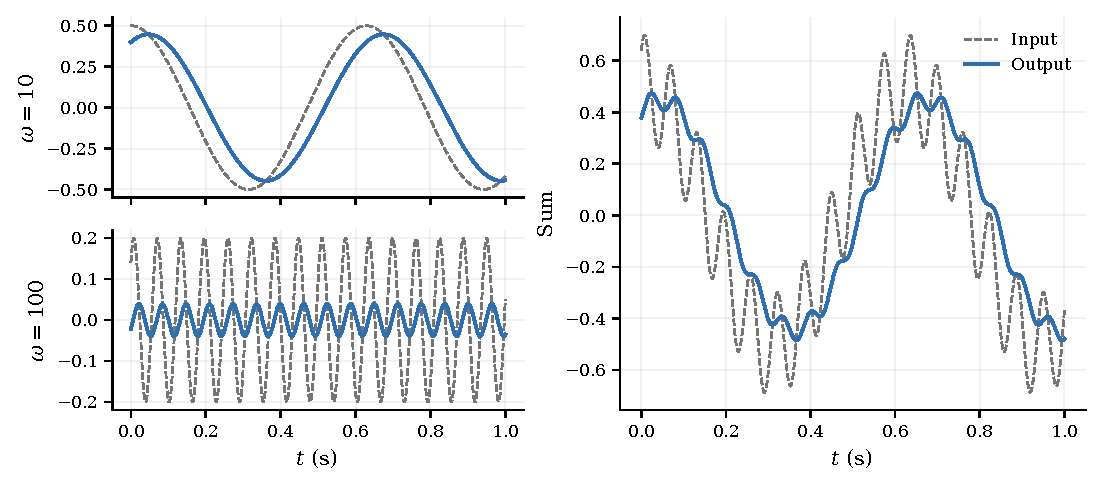
\includegraphics[width=.98\linewidth]{ch5-lowpass-example.pdf}
\end{center}
高频分量被明显抑制，输出主要由低频项决定。高、低频幅值比由 $0.2/0.5=0.4$ 变为约 $0.087706$；各分量相对强弱改变，叠加波形不能只用共同放大与延迟表示。

两分量的等效相位延迟也不同：
\[
t_1=\frac{\arctan0.5}{10}\approx0.046365\,\mathrm s,\qquad
t_2=\frac{\arctan5}{100}\approx0.013734\,\mathrm s.
\]
本滤波器截止角频率 $\omega_c=1/\tau=20\,\mathrm{rad/s}$，截止频率约 $3.1831\,\mathrm{Hz}$。输入高频项处于截止点之上，所以衰减显著。

\subsection*{本题知识点与公式}\label{kn:5-6}
\noindent\textbf{已学前置：}一阶系统的微分方程、传递函数、冲激/阶跃响应和幅相特性见\hyperref[kn:3-1]{第3章第1题}；误差与带宽见\hyperref[kn:3-2]{第3章第2题}；相位延迟、群延迟见\hyperref[kn:3-4]{第3章第4题}。本题保留逐频率解法，新增RC实现、实际加载与级联，以及滤波时如何评价多频保真。

\paragraph{1. 一个RC电路怎样实现题给频响}
理想电压源经电阻 $R$ 接到输出节点，电容 $C$ 从输出接地；输出取电容两端、负载开路。电容阻抗 $Z_C=1/(sC)$，由串联分压，
\[
H(s)=\frac{Z_C}{R+Z_C}=\frac1{1+sRC}.
\]
因此 $\tau=RC$，$R$ 以 $\Omega$ 计、$C$ 以F计、$\tau$ 以s计。本题给出的 $\tau=0.05\,\mathrm s$ 只规定乘积，不能唯一反推出 $R,C$ 各自数值。低频时电容阻抗大、输出接近输入；高频时电容阻抗小、输出被旁路到地，解释了其低通性质。若输出改取电阻两端，频响变为 $sRC/(1+sRC)$，实现高通而非本题模型。

\paragraph{2. 有限负载会同时改变直流增益和时间常数}
若输出端并联纯电阻负载 $R_L$，其等效阻抗为
$Z_p=R_L/(1+sR_LC)$，因此
\[
\boxed{
H_L(s)=
\frac{R_L}{R+R_L}\,
\frac1{1+s(R\parallel R_L)C}
}.
\]
实际直流增益 $K_L=R_L/(R+R_L)$ 小于1，实际时间常数为 $(R\parallel R_L)C$，二者都与未加载结果不同。不能只看到截止频率升高就说测量更准确，因为电压已经先被分压衰减。理想源若有串联内阻 $R_s$，式中驱动电阻应换为 $R+R_s$；若负载还含电容或频率相关阻抗，需重新列网络方程。

要使用本题给定的单位静态增益模型，实际电路须已标定且可用此模型描述，或满足驱动阻抗足够小、负载阻抗远大于所用电阻。电压跟随器等缓冲级以高输入阻抗减小前级加载、以低输出阻抗驱动后级；缓冲器自身带宽与增益误差仍须足够小。

\paragraph{3. 级联后不能沿用单级的截止点}
有缓冲、级间加载可忽略时，总频响是各级复频响的乘积。$N$ 个相同一阶低通级联，
\[
H_N(s)=(1+s\tau)^{-N},\qquad
A_N(\omega)=[1+(\omega\tau)^2]^{-N/2},
\]
\[
\phi_N(\omega)=-N\arctan(\omega\tau).
\]
总幅值相乘、相位相加；它并不等价于把单级 $\tau$ 机械换成 $N\tau$。按总直流增益的半功率点定义截止，解 $A_N=1/\sqrt2$ 得
\[
\boxed{f_{c,N}=\frac{\sqrt{2^{1/N}-1}}{2\pi\tau}}.
\]
$N>1$ 时总体截止低于单级截止。级联虽使高频抑制更强，也会改变通带衰减与相位，所以必须重新核对基带精度。

若两个相同的无源RC低通直接串接、没有缓冲，后一段会加载前一段。设一级节点为 $V_1$、最终输出为 $V_o$，理想电压源为 $V_{\mathrm{in}}$。零初值、最终开路时，节点电流守恒给出
\[
\frac{V_{\mathrm{in}}-V_1}{R}=sCV_1+\frac{V_1-V_o}{R},
\qquad \frac{V_1-V_o}{R}=sCV_o.
\]
由第二式得 $V_1=(1+sRC)V_o$，代入第一式并整理，得到
\[
H_{\mathrm{unbuf}}(s)=\frac1{1+3sRC+s^2R^2C^2},
\]
而非 $(1+sRC)^{-2}$。这个差别说明乘积法的前提是\textbf{各级在实际连接条件下的频响已知}，不是只要画出两个模块就能乘各自空载频响。

\paragraph{4. 多频保真要比较相对幅值和延迟}
设输入为 $\sum_iX_i\cos(\omega_it+\theta_i)$，输出逐项乘 $A_i$、加 $\phi_i$。若目标是保留整个波形，应在有效频带内近似满足
\[
H(\iu\omega)\approx A_0e^{-\iu\omega t_0},
\]
即同一个幅值比 $A_0$ 与同一个延迟 $t_0$，不能只要求每项频率不变。本题高低频幅值比由0.4变为约0.087706，已说明相对强弱明显改变；两个系统新增相位也不对应同一相位延迟。

依\hyperref[kn:3-4]{第3章第4题的延迟定义}，对本题RC直接代入得
\[
t_\phi(\omega)=\frac{\arctan(\omega\tau)}{\omega},
\qquad
\tau_g(\omega)=\frac{\tau}{1+(\omega\tau)^2}.
\]
两者单位为s，求导或计算时相位用rad。前者对应单频相位的等效延迟，后者反映足够窄频带附近包络的传播延迟；不能互相替代。只有 $\omega\tau\ll1$ 时二者都近似 $\tau$。本题 $\omega\tau=0.5$ 与5，相位延迟分别为答案中的0.046365 s与0.013734 s；群延迟则分别为0.04 s与约0.001923 s，也并非常数。

\paragraph{5. 低通的抑噪收益与失真代价}
增大 $\tau$ 会降低截止频率，使高频衰减和相位滞后更强。本题 $\tau$ 是第\ref{hw:3-1}节的10倍；若 $100\,\mathrm{rad/s}$ 分量也属被测信号，输出已不保真。若只提取低频，仍须核查低频项约 $10.56\%$ 的衰减。应先定有用频带与允许幅相误差，再选 $\tau$、阶次和标定；同频干扰不能靠选频滤波无损分离。

\nt{这里 $\tau=0.05\,\mathrm s$，应直接代入本题参数。求的是稳定滤波后的稳态输出，不含启动暂态；若要求从零初始状态接入信号后的全过程，还应依据初始条件补上 $Ce^{-t/\tau}$。}
